\documentclass{article}
\usepackage[spanish]{babel}
\usepackage[utf8]{inputenc}
\usepackage{graphicx}
\usepackage{minted}
\usepackage{courier}
\usepackage[dvipsnames]{xcolor}
\usepackage{relsize}

\definecolor{red}{rgb}{0.95,0.12,0.14}
\definecolor{green}{rgb}{0.47,0.58,0.17}
\definecolor{darkTurquoise}{rgb}{0.18,0.65,0.74}
\definecolor{blue}{rgb}{0.16,0,0.98}
\definecolor{purple}{rgb}{0.65,0.03,0.69}

\title{\textbf{Criptografía aplicada: Cálculo del hash SHA-256 de un bloque Bitcoin}}
\author{Javier Domínguez Gómez \\
\small{jdg@member.fsf.org} \\
\small{Fingerprint: 94AD 19F4 9005 EEB2 3384 C20F 5BDC C668 D664 8E2B}}
\date{v0.1.03 - Febrero 2019}

\begin{document}
\maketitle

\tableofcontents{}

\section{Introducción}
    Este documento describe en detalle cada una de las partes de las que se compone un bloque en la cadena de bloques de Bitcoin. También describe el tipo y la distribución de los datos en el bloque, así como las operaciones lógico-matemáticas de la función criptográfica SHA-256 que se emplean con el fin de generar el \textit{hash} adecuado que finalmente representará dicho bloque en la cadena de bloques.

\section{Estructura de datos de un bloque}
    \vspace{3mm}
    Cada bloque de la cadena de bloques de Bitcoin se compone de una serie de datos ordenados meticulosamente y con una lógica definida que se explicará en los siguientes puntos. Cada uno de estos datos tiene sus propios atributos, como puede ser el tipo de dato, el nombre, el tamaño que ocupa en memoria y el formato en el que este se representará. En la siguiente tabla se categorizan los más significativos.
    \begin{table}[H]
    \centering
    \begin{tabular}{| c | l | c | l |} 
        \hline
        Tipo de dato & Nombre & Tamaño & Formato \\
        \hline
        uint32\_t & magicID & 4 bytes & Little-endian \\
        \hline
        uint32\_t & headerLenght & 4 bytes & Big-endian \\
        \hline
        uint32\_t & versionNumber & 4 bytes & Little-endian \\
        \hline
        uint8\_t[32] & previousBlockHash & 32 bytes & Big-endian \\
        \hline
        uint8\_t[32] & merkleRoot & 32 bytes & Big-endian \\
        \hline
        uint32\_t & timeStamp & 4 bytes & Little-endian \\
        \hline
        uint32\_t & targetDifficulty & 4 bytes & Little-endian \\
        \hline
        uint32\_t & nonce & 4 bytes & Little-endian \\
        \hline
        uint8/16/32/64\_t & transactionCount & 1, 3, 5 o 9 bytes & Big-endian*  \\
        \hline
    \end{tabular}
    \caption{Principales datos de un bloque en la cadena de bloques de Bitcoin.}
    \label{table:0}
    \end{table}
    
    \begin{enumerate}
        \item \textbf{magicID}: En la red de Bitcoin se establecen conexiones entre los nodos con la finalidad de establecer una comunicación para el envío y recepción de datos o mensajes. Los mensajes se envían mediante un canal en el que según van llegando se van concatenando uno detrás de otro. Así pues, cuando se desarrolló el protocolo Bitcoin se vio conveniente añadir un prefijo en cada mensaje anteponiendo este dato de 4 bytes y así poder identificar fácilmente no solo la red de Bitcoin en la que se generan, si no también dónde empieza y termina cada mensaje que circula entre los diferentes nodos de la red. La siguiente tabla muestra los diferentes valores que puede tener la variable \textit{magicID} dependiendo de la red.
        
        \begin{table}[H]
        \centering
        \begin{tabular}{| c | c |} 
            \hline
            Red & magicID \\
            \hline
            Mainnet & \texttt{0xf9beb4d9} \\
            \hline
            Testnet & \texttt{0xfabfb5da} \\
            \hline
            Testnet3 & \texttt{0x0b110907} \\
            \hline
            Namecoin & \texttt{0xf9beb4fe} \\
            \hline
            Regtest & \texttt{0xfabfb5da} \\
            \hline
        \end{tabular}
        \label{table:1}
        \end{table}
        
        Se decidió establecer estos valores tan específicos dada la improbabilidad de que los caracteres ASCII que representan se encuentren en un mensaje estándar, tal y como se indica en el archivo \textit{chainparams.cpp}\footnote{https://github.com/bitcoin/bitcoin/blob/master/src/chainparams.cpp\#L99} que lo implementa en el código de Bitcoin.
    
        \item \textbf{headerLenght}: En un dato numérico hexadecimal de 4 bytes y de valor variable que representa la longitud en bytes del bloque actual. Está codificado en formato \textit{Big-endian}
        
        \item \textbf{versionNumber}: Este dato hexadecimal puede cambiar de valor cuando se actualiza el software y cambia el número de la versión del protocolo. Se codifica en formato \textit{Little-endian}.
        
        \item \textbf{previousBlockHash}: Se trata del \textit{hash} o \textit{digest} resultante del bloque anterior tras aplicar las funciones criptográficas utilizando los datos de la cabecera de dicho bloque. Tiene una longitud de 256 bits o 32 bytes codificado en formato \textit{Big-endian}.
        
        \item \textbf{merkleRoot}: Cada vez que una nueva transacción es aceptada el valor de esta variable se modifica. Se trata de un \textit{hash} hexadecimal de 32 bytes codificado en formato \textit{Big-endian}. Para obtener el \textit{hash} final, también llamado \textit{hash root} se han de concatenar los datos de las transacciones ubicados en los nodos hoja del árbol, en grupos de dos. De ese modo, por cada dos transacciones se obtiene un \textit{hash} nuevo que será incluido en un nuevo vector que repetirá la acción hasta llegar al \textit{hash root}.
        
        \begin{figure}[H]
        \centering
            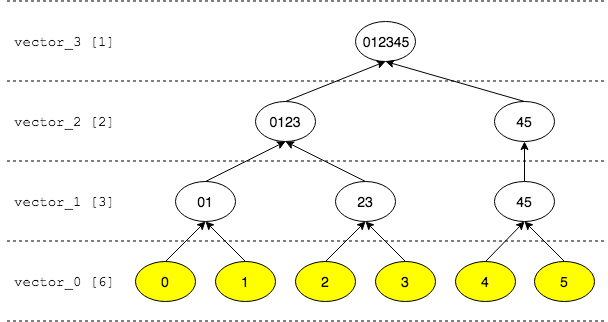
\includegraphics[scale=0.53]{img/Merkle_tree_05_leaves_nodes}
            \caption{Ejemplo de árbol de Merkle con 5 nodos hoja}
        \end{figure}
        
        Cada uno de los vectores $\mathbf{v} \ = \langle v_{1}, v_{2}, \dots, v_{n - 1}, v_{n} \rangle$ irá reduciendo el numero de nodos o elementos mediante la siguiente función recursiva por intervalos o algoritmo de complejidad $O(n)$.
        
        \begin{figure}[H]
        \centering
            $f(\mathbf{v}) = \mathlarger{\sum}_{i=0}^{n} \left \{
            \begin{array}{ll}
                \langle \mathbf{v}^{\prime}, v_{i}\rangle & \mbox{si } i=n-1 \\
                \langle \mathbf{v}^{\prime}, v_{i}||v_{i+1} \rangle & \mbox{si } i < n \\
                i+2
            \end{array}
            \right .$
        \end{figure}
        A continuación un ejemplo escrito en lenguaje C++ que implementa dicho algoritmo:
        
        \begin{minted}[fontsize=\small]{cpp}
#include <iostream>
#include <sstream>
#include <vector>
#include "sha256.h"
 
using namespace std;
 
void printVector(vector<string>);
string merkleTree(vector<string>);
string merkleTreeRoot;
 
int main(int argc, char *argv[]) {
    string msg = argv[1];
    istringstream buf(msg);
    vector<string> leafNodesV;
    
    for (string node; buf >> node;)
        leafNodesV.push_back(sha256(node));
        
    printVector(leafNodesV);
    cout << "Root: " << merkleTree(leafNodesV) << endl;
    
    return 0;
}

string merkleTree(vector<string> v) {
    if (v.size() > 1) {
        vector<string> aux;
        int i;
        
        for (i = 0; i < v.size(); i += 2) {
            if (i == v.size() - 1) {
                aux.push_back(v[i]);
            } else if (i < v.size()) {
                aux.push_back(sha256(v[i] + v[i + 1]));
            }
        }
        merkleTree(aux);
    } else if(v.size() == 1){
        merkleTreeRoot = v[0];
    }
    
    return merkleTreeRoot;
}

void printVector(vector<string> v) {
    cout << "v.size() = " << v.size() << endl;
    int i = 0;
    while (i < v.size()) {
        cout << "v[" << i << "]: " << v[i] << endl;
        i++;
    }
}
        \end{minted}
        
        \item \textbf{timeStamp}: Se trata de un número entero sin signo de 4 bytes también llamado \textit{Epoch} o \textit{Tiempo Unix}. Representa el número de segundos que han transcurrido desde el 1 de enero de 1970 a las 00:00. Se codifica en formato \textit{Little-endian}.
        
        Un ejemplo de cómo se puede calcular este dato es mediante el siguiente código C. Nótese que las horas se procesan como \textit{GMT+1}.
        
        \begin{minted}[fontsize=\small]{c}
#include <stdio.h>
#include <time.h>

int main(int argc, char *argv[]) {
    int year, month, day, hour, minute, second;
    struct tm t;
    time_t tod;
    
    printf("Year: ");
    scanf("%d", &year);
    printf("Month: ");
    scanf("%d", &month);
    printf("Day: ");
    scanf("%d", &day);
    printf("Hour: ");
    scanf("%d", &hour);
    printf("Minute: ");
    scanf("%d", &minute);
    printf("Second: ");
    scanf("%d", &second);
    
    t.tm_year = year - 1900;
    t.tm_mon = month - 1;   // Values [0-11]
    t.tm_mday = day;
    t.tm_hour = hour + 1;   // GMT+1
    t.tm_min = minute;
    t.tm_sec = second;
    t.tm_isdst = 0;         // DST = 0
    tod = mktime(&t);
    
    printf("Timestamp epoch: %ld\n", (long) tod);
}
        \end{minted}
        
    
        \item \textbf{targetDifficulty}: Se trata de un número entero de 256 bits representado como un número decimal muy grande, tanto que abarcaría el rango de números existentes entre $0$ y $2^{256}-1$. Su función es la de definir una variable más a tener en cuenta a la hora de obtener el hash adecuado de un bloque antes de ser minado. Así pues la prueba de trabajo o \textit{Proof of Work} tendrá mayor o menor dificultad. En el protocolo de Bitcoin se define una regla que dice que el \textit{hash} del bloque ha de ser un número menor o igual al valor de la variable \textit{targetDifficulty} en ese momento. Así pues, si el \textit{hash} obtenido como candidato a generar un bloque fuera un número menor o igual al de \textit{targetDifficulty} habría posibilidades para que el \textit{hash} candidato sea un \textit{hash} válido para generar un nuevo bloque, aunque de forma adicional se han de cumplir otras condiciones. Por el contrario, si el \textit{hash} obtenido como candidato fuera un número mayor que el valor de la variable \textit{targetDifficulty}, se ha de incrementar el valor de la variable \textit{nonce} y probar otra vez a generar un \textit{hash} nuevo.
        
        \begin{figure}[H]
        \centering
            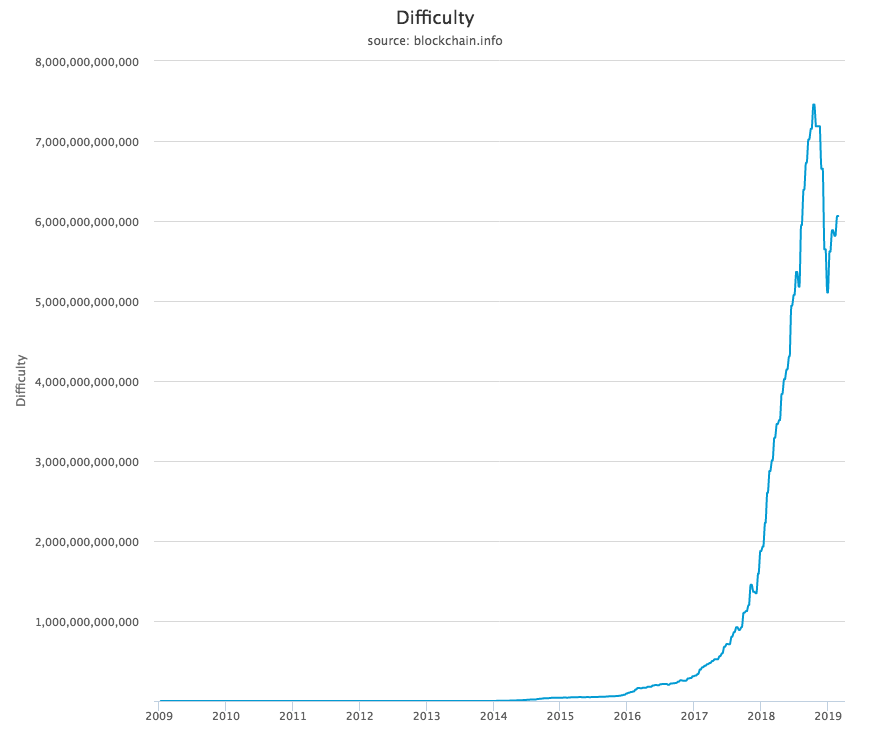
\includegraphics[scale=0.39]{img/Bitcoin_TargetDifficulty.png}
            \caption{Valor de la variable \textit{targetDifficulty} desde enero de 2009 hasta hoy.}
        \end{figure}
        
        El valor de la variable \textit{targetDifficulty} se modifica automáticamente una vez se han generado 2016 bloques, esto sucede aproximadamente cada dos semanas. El nuevo valor se obtiene mediante un cálculo que realizan todos los clientes Bitcoin de la red en el que toman el tiempo real que ha llevado generar los 2016 bloques y se obtiene la diferencia porcentual respecto al número de bloques que se esperaba haber calculado en el periodo de dos semanas.
        
        \item \textbf{nonce}: Se trata de un número entero sin signo aleatorio con una longitud de 32 bits o 4 bytes codificado en formato \textit{Little-endian}. Es el dato que ha de cambiarse tras un intento fallido por encontrar el hash del bloque adecuado, de modo que se incrementa y se han de realizar de nuevo todos los cálculos criptográficos teniendo en cuenta el nuevo valor de esta variable.
        
        \item \textbf{transactionCount}: En el caso de \textit{transactionCount} el tipo de dato es un entero sin signo de longitud variable. Como el propio nombre indica, dependiendo del número de transacciones que han sido procesadas tendrá un valor numérico u otro.
        
        *Cuando se le asigna por valor un entero muy grande se codifica en formato \textit{Little-endian}.
    \end{enumerate}
    
    \begin{figure}[H]
    \centering
        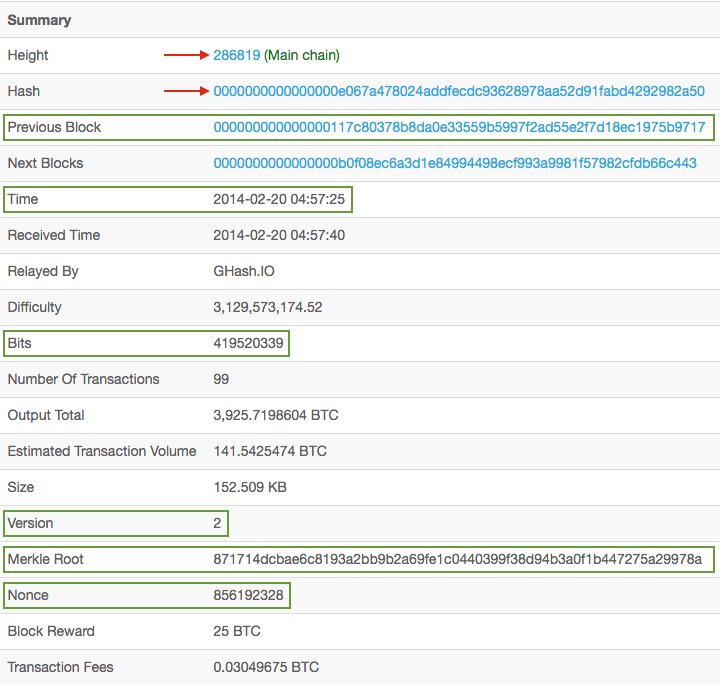
\includegraphics[scale=0.47]{img/Bitcoin_block_SHA_256_Block_Data}
        \caption{Datos empleados para la obtención del \textit{hash} del bloque \#$286819$.}
    \end{figure}
    
    \vspace{3mm}

\section{Almacenamiento en ficheros}
    Así es como se ven los datos de un bloque almacenados en un fichero blk*.dat.
    \begin{figure}[H]
    \scriptsize{\texttt{$\sim\$$ hexdump\ -C\ -s\ 93725126\ -n\ 288\ blk00116.dat}}
    
    \scriptsize{
    \texttt{059621c6  \textbf{\textcolor{red}{f9 be b4 d9} \textcolor{green}{bd 53 02 00}  \textcolor{darkTurquoise}{02 00 00 00 17 97 5b 97}}  |.....S........[.|} \\
    \texttt{059621d6  \textbf{\textcolor{darkTurquoise}{c1 8e d1 f7 e2 55 ad f2  97 59 9b 55 33 0e da b8}}  |.....U...Y.U3...|} \\
    \texttt{059621e6  \textbf{\textcolor{darkTurquoise}{78 03 c8 17 01 00 00 00  00 00 00 00 8a 97 29 5a}}  |x.............)Z|} \\
    \texttt{059621f6  \textbf{\textcolor{darkTurquoise}{27 47 b4 f1 a0 b3 94 8d  f3 99 03 44 c0 e1 9f a6}}  |'G.........D....|} \\
    \texttt{05962206  \textbf{\textcolor{darkTurquoise}{b2 b9 2b 3a 19 c8 e6 ba  dc 14 17 87 35 8b 05 53}}  |..+:........5..S|} \\
    \texttt{05962216  \textbf{\textcolor{darkTurquoise}{53 5f 01 19 48 75 08 33}  \textcolor{blue}{63} \textcolor{purple}{01 00 00 00 01 00 00}}  |S\_..Hu.3c.......|} \\
    \texttt{05962226  \textbf{\textcolor{purple}{00 00 00 00 00 00 00 00  00 00 00 00 00 00 00 00}}  |................|} \\
    \texttt{05962236  \textbf{\textcolor{purple}{00 00 00 00 00 00 00 00  00 00 00 00 00 00 ff ff}}  |................|} \\
    \texttt{05962246  \textbf{\textcolor{purple}{ff ff 60 03 63 60 04 06  2f 50 32 53 48 2f 04 35}}  |..`.c`../P2SH/.5|} \\
    \texttt{05962256  \textbf{\textcolor{purple}{8b 05 53 08 44 04 f2 53  00 00 17 e4 46 52 2c fa}}  |..S.D..S....FR,.|} \\
    \texttt{05962266  \textbf{\textcolor{purple}{be 6d 6d 69 06 88 fb 88  6c 0d f0 c8 7c bc 7e a4}}  |.mmi....l...|.~.|} \\
    \texttt{05962276  \textbf{\textcolor{purple}{f7 f1 b5 c0 05 0b d0 ac  37 51 cf c9 97 d9 d6 97}}  |........7Q......|} \\
    \texttt{05962286  \textbf{\textcolor{purple}{13 28 de 04 00 00 00 00  00 00 00 48 61 70 70 79}}  |.(.........Happy|} \\
    \texttt{05962296  \textbf{\textcolor{purple}{20 4e 59 21 20 59 6f 75  72 73 20 47 48 61 73 68}}  | NY! Yours GHash|} \\
    \texttt{059622a6  \textbf{\textcolor{purple}{2e 49 4f 00 00 00 00 01  cb 81 31 95 00 00 00 00}}  |.IO.......1.....|} \\
    \texttt{059622b6  \textbf{\textcolor{purple}{19 76 a9 14 80 ad 90 d4  03 58 1f a3 bf 46 08 6a}}  |.v.......X...F.j|} \\
    \texttt{059622c6  \textbf{\textcolor{purple}{91 b2 d9 d4 12 5d b6 c1  88 ac 00 00 00 00 01 00}}  |.....]..........|} \\
    \texttt{059622d6  \textbf{\textcolor{purple}{00 00 01 7d 67 7c de 17  3f 8c bf 43 31 27 a8 5e}}  |...\}g|..?..C1'.\textasciicircum|}
    }
    \end{figure}
    
\section{Construcción de la cadena de entrada M}
    En este ejemplo se tratarán los datos reales del bloque $\#286819$ de la cadena de bloques de Bitcoin. Este bloque tiene el siguiente \textit{hash}.
    
    \begin{figure}[H]
        \centering
        \scriptsize{
        \texttt{0000000000000000e067a478024addfecdc93628978aa52d91fabd4292982a50}
        }
    \end{figure}
    
    Los datos correspondientes a la cabecera o \textit{header} son los siguientes:
    \begin{figure}[H]
    \centering
    \scriptsize{
        $\begin{array}{ll}
            \texttt{Version:} & \texttt{2} \\
            \texttt{Prev. Block:} & \texttt{000000000000000117c80378b8da0e33559b5997f2ad55e2f7d18ec1975b9717} \\
            \texttt{Merkle root:} & \texttt{871714dcbae6c8193a2bb9b2a69fe1c0440399f38d94b3a0f1b447275a29978a} \\
            \texttt{Timestamp:} & \texttt{2014-02-20 04:57:25 (Epoch timestamp: 1392872245)} \\
            \texttt{Bits:} & \texttt{419520339} \\
            \texttt{Nonce:} & \texttt{856192328} \\
        \end{array}$
    }
    \end{figure}
    
    Pasamos los datos decimales a formato hexadecimal:
    \begin{figure}[H]
    \centering
    \scriptsize{
        $\begin{array}{ll}
            \texttt{Version:} & \texttt{00000002} \\
            \texttt{Prev. Block:} & \texttt{000000000000000117c80378b8da0e33559b5997f2ad55e2f7d18ec1975b9717} \\
            \texttt{Merkle root:} & \texttt{871714dcbae6c8193a2bb9b2a69fe1c0440399f38d94b3a0f1b447275a29978a} \\
            \texttt{Timestamp:} & \texttt{53058B35} \\
            \texttt{Bits:} & \texttt{19015F53} \\
            \texttt{Nonce:} & \texttt{33087548} \\
        \end{array}$
    }
    \end{figure}
    
    Se reorganizan los datos en formato Little Endian:
    \begin{figure}[H]
    \centering
    \scriptsize{
        $\begin{array}{ll}
            \texttt{Version:} & \texttt{02000000} \\
            \texttt{Prev. Block:} & \texttt{17975b97c18ed1f7e255adf297599b55330edab87803c8170100000000000000} \\
            \texttt{Merkle root:} & \texttt{8a97295a2747b4f1a0b3948df3990344c0e19fa6b2b92b3a19c8e6badc141787} \\
            \texttt{Timestamp:} & \texttt{358B0553} \\
            \texttt{Bits:} & \texttt{535F0119} \\
            \texttt{Nonce:} & \texttt{48750833} \\
        \end{array}$
    }
    \end{figure}
    
    Finalmente se concatenan uno a continuación de otro, empezando por versión, hash del bloque anterior, merkle root, timestamp, bits y nonce, formando una cadena de entrada $M$ de 160 carácteres hexadecimales con con un tamaño total de 640 bits.
    
    \begin{figure}[H]
    \centering
        $\begin{array}{rcl}
             M & = & \left \{
            \begin{array}{c}
                \texttt{0200000017975b97c18ed1f7e255adf2} \\
                \texttt{97599b55330edab87803c81701000000} \\
                \texttt{000000008a97295a2747b4f1a0b3948d} \\
                \texttt{f3990344c0e19fa6b2b92b3a19c8e6ba} \\
                \texttt{dc141787358b0553535f011948750833}
            \end{array}
            \right .
        \end{array}$
    \end{figure}
    
    Se segmenta la cadena de entrada $M$ en bloques de 32 bits:
    \begin{figure}[H]
    \centering
        $\begin{array}{rcl}
             M & = & \left \{
            \begin{array}{c}
                \texttt{02000000 + 17975b97 + c18ed1f7 + e255adf2} \\
                \texttt{97599b55 + 330edab8 + 7803c817 + 01000000} \\
                \texttt{00000000 + 8a97295a + 2747b4f1 + a0b3948d} \\
                \texttt{f3990344 + c0e19fa6 + b2b92b3a + 19c8e6ba} \\
                \texttt{dc141787 + 358b0553 + 535f0119 + 48750833}
            \end{array}
            \right .
        \end{array}$
    \end{figure}

\section{Longitud de la cadena $M$ de entrada}
    Una vez que se ha obtenido la cadena de entrada $M$ en el punto anterior es necesario calcular la longitud de la misma en formato hexadecimal o base 16, es decir, 640 bits que se representan con el valor 280 en hexadecimal.
    \begin{figure}[H]
    \centering
        $|M| = 280\ (640\ bits\ del\ mensaje\ original\ en\ hexadecimal)$
    \end{figure}
    Este dato se ha de reservar para el siguiente punto, ya que será necesario para completar los registros $W_{14}$ y $W_{15}$ de la variable $W_t$ solo en la segunda y tercera ejecución de la función SHA-256.
    
\section{Los 16 registros de $W_t$}
    En la siguiente figura se detalla el contenido de los primeros 16 registros de la variable $W_{t}$ en cada una de las tres veces que se ejecutan las 64 iteraciones de la función SHA-256 para obtener el \textit{digest} en cada caso.
    \begin{figure}[H]
    \centering
        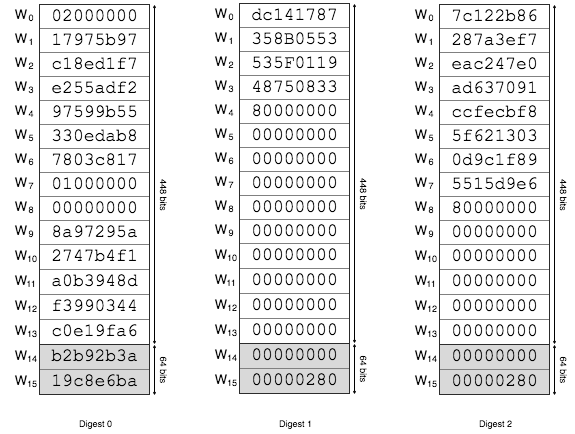
\includegraphics[scale=0.59]{img/Bitcoin_block_SHA_256_W0_W15_x3}
        \caption{Los primeros 16 registros de la variable $W_{t}$ en los tres casos en los que se ha de ejecutar la función SHA-256.}
    \end{figure}
    
    \subsection{Primera ronda SHA-256: Ronda 0}
    La función \textit{hash} SHA-256 realiza 64 ciclos criptográficos en los que procesará una serie de cálculos en los que tiene en cuenta por un lado las 8 palabras hexadecimales de 32 bits asignadas como valor a las variables $A$, $B$, $C$, $D$, $E$, $F$, $G$ y $H$, y por otro lado la variable $W_t$, que es un vector de 64 elementos ordenados por intervalos. En esta primera ronda criptográfica se han iniciar los valores de las variables $A_{0}$, $B_{0}$, $C_{0}$, $D_{0}$, $E_{0}$, $F_{0}$, $G_{0}$ y $H_{0}$ con los valores estándar de la función \textit{hash} SHA-256 en su primera iteración, es decir, los 32 primeros bits en hexadecimal o base 16 de la parte fraccionaria de las raíces cuadradas de los primeros 8 números primos.
    
    \begin{figure}[H]
    \centering
        $\begin{array}{ll}
            A_{0} = \texttt{0x6a09e667} & B_{0} = \texttt{0xbb67ae85} \\
            C_{0} = \texttt{0x3c6ef372} & D_{0} = \texttt{0xa54ff53a} \\
            E_{0} = \texttt{0x510e527f} & F_{0} = \texttt{0x9b05688c} \\
            G_{0} = \texttt{0x1f83d9ab} & H_{0} = \texttt{0x5be0cd19}
        \end{array}$
    \end{figure}
    Los primeros 16 elementos del vector $W_t$ se han de rellenar con los primeros 512 bits de la cadena principal de entrada $M$, tal y como se muestra en la imagen.
    
    \begin{figure}[H]
        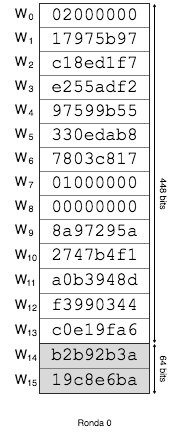
\includegraphics[scale=0.59]{img/Bitcoin_block_SHA_256_W0_W15_ronda_0}
    \end{figure}
    
    \subsection{Segunda ronda SHA-256: Ronda 1}
    \begin{figure}[H]
    \centering
        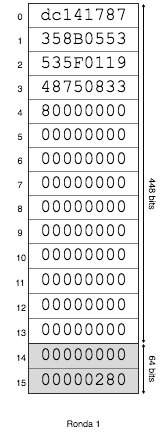
\includegraphics[scale=0.59]{img/Bitcoin_block_SHA_256_W0_W15_ronda_1}
    \end{figure}
    
    \subsection{Tercera ronda SHA-256: Ronda 2}
    \begin{figure}[H]
    \centering
        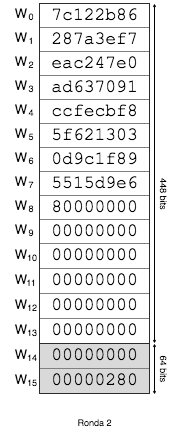
\includegraphics[scale=0.59]{img/Bitcoin_block_SHA_256_W0_W15_ronda_2}
    \end{figure}
\end{document}
